\documentclass[tikz,border=2pt]{standalone}
\usepackage{amsmath}
\usepackage[T1]{fontenc}
\usepackage{XCharter}
\usepackage[xcharter,vvarbb]{newtxmath}
\usetikzlibrary{arrows.meta,calc,positioning,fit,backgrounds}
\definecolor{ink}{HTML}{222222}
\definecolor{cb}{HTML}{0072B2}
\definecolor{co}{HTML}{E69F00}
\definecolor{cs}{HTML}{56B4E9}
\newcommand{\sm}{\fontsize{6.5}{7.4}\selectfont}
\tikzset{
  every node/.style={font=\fontsize{7.2}{8.3}\selectfont, text=ink},
  layer/.style={draw=ink, rounded corners=1.6pt, line width=0.5pt, fill=cs!16, align=center, inner sep=2.2pt},
  opt/.style={layer, dashed, dash pattern=on 2pt off 1.4pt, fill=white},
  turn/.style={draw=ink, line width=0.4pt, minimum size=0.26cm, inner sep=0pt},
  ent/.style={circle, draw=ink, line width=0.4pt, minimum size=0.2cm, inner sep=0pt, fill=co!40},
  arr/.style={-{Stealth[length=3.2pt,width=2.6pt]}, line width=0.5pt, draw=ink},
  darr/.style={arr, densely dashed},
  edge/.style={line width=0.35pt, draw=ink!70},
  frame/.style={draw=ink!50, rounded corners=2.5pt, line width=0.4pt, inner sep=3.5pt},
  ttl/.style={font=\fontsize{7.8}{8.8}\selectfont\bfseries, anchor=west},
}
\begin{document}
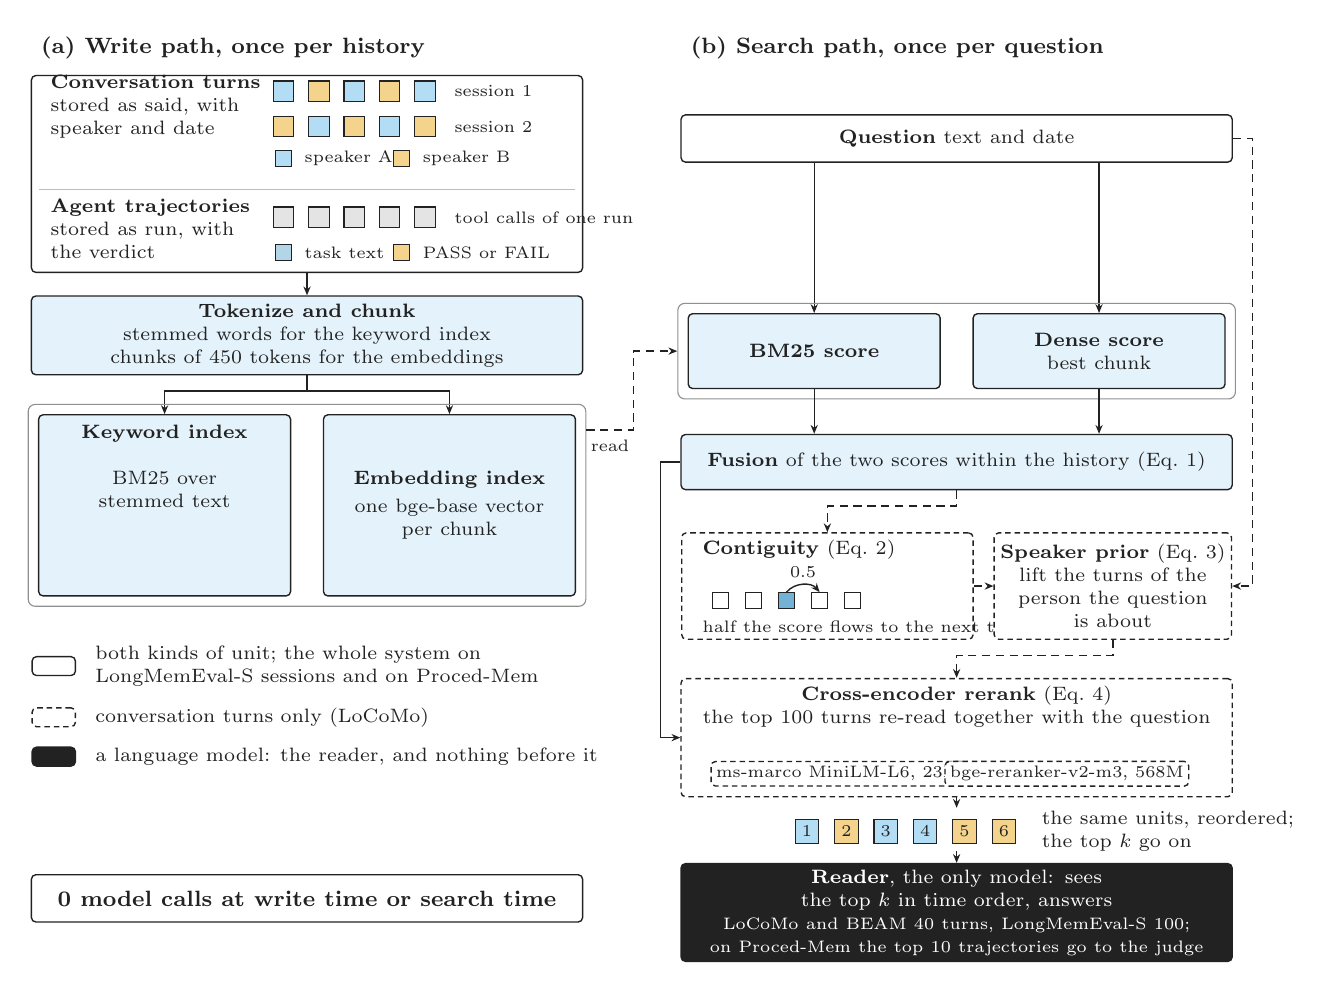
\begin{tikzpicture}[x=1cm,y=1cm]
\def\LX{3.5}
\def\RX{11.75}
\def\W{7.0}
\def\BW{2.2}
\def\IY{-3.35}
\def\RY{-2.55}

\node[ttl] at (\LX-\W/2,1.3) {(a) Write path, once per history};
\node[ttl] at (\RX-\W/2,1.3) {(b) Search path, once per question};

% ================= (a) =================
\node[layer, fill=white, minimum width=\W cm, minimum height=2.5cm] (hist) at (\LX,-0.3) {};
\node[anchor=west, align=left] at (\LX-\W/2+0.12,0.55) {\textbf{Conversation turns}\\stored as said, with\\speaker and date};
\foreach \i/\c in {0/cs,1/co,2/cs,3/co,4/cs} { \node[turn, fill=\c!45] at (\LX-0.3+0.45*\i,0.75) {}; }
\foreach \i/\c in {0/co,1/cs,2/co,3/cs,4/co} { \node[turn, fill=\c!45] at (\LX-0.3+0.45*\i,0.3) {}; }
\node[anchor=west, font=\sm] at (\LX+1.75,0.75) {session 1};
\node[anchor=west, font=\sm] at (\LX+1.75,0.3) {session 2};
\node[turn, fill=cs!45, minimum size=0.2cm] (sa) at (\LX-0.3,-0.1) {};
\node[anchor=west, font=\sm] at ($(sa.east)+(0.04,0)$) {speaker A};
\node[turn, fill=co!45, minimum size=0.2cm] (sb2) at (\LX+1.2,-0.1) {};
\node[anchor=west, font=\sm] at ($(sb2.east)+(0.04,0)$) {speaker B};
\draw[edge, ink!30] (\LX-\W/2+0.1,-0.5) -- (\LX+\W/2-0.1,-0.5);
\node[anchor=west, align=left] at (\LX-\W/2+0.12,-1.0) {\textbf{Agent trajectories}\\stored as run, with\\the verdict};
\foreach \i in {0,1,2,3,4} { \node[turn, fill=ink!12] at (\LX-0.3+0.45*\i,-0.85) {}; }
\node[anchor=west, font=\sm] at (\LX+1.75,-0.85) {tool calls of one run};
\node[turn, fill=cb!30, minimum size=0.2cm] (pv) at (\LX-0.3,-1.3) {};
\node[anchor=west, font=\sm] at ($(pv.east)+(0.04,0)$) {task text};
\node[turn, fill=co!45, minimum size=0.2cm] (pv2) at (\LX+1.2,-1.3) {};
\node[anchor=west, font=\sm] at ($(pv2.east)+(0.04,0)$) {PASS or FAIL};
\node[layer, minimum width=\W cm, minimum height=1.0cm] (parse) at (\LX,-2.35) {\textbf{Tokenize and chunk}\\stemmed words for the keyword index\\chunks of 450 tokens for the embeddings};
\draw[arr] (hist.south) -- (parse.north);

\node[layer, minimum width=3.2cm, minimum height=2.3cm, anchor=north east] (bm) at (\LX-0.2,\IY) {};
\node at ($(bm.north)+(0,-0.25)$) {\textbf{Keyword index}};
\node[align=center] at ($(bm.north)+(0,-0.95)$) {BM25 over\\stemmed text};

\node[layer, minimum width=3.2cm, minimum height=2.3cm, anchor=north west] (de) at (\LX+0.2,\IY) {\textbf{Embedding index}\\[2pt]one bge-base vector\\per chunk};

\draw[arr] (parse.south) -- ++(0,-0.2) -| (bm.north);
\draw[arr] (parse.south) -- ++(0,-0.2) -| (de.north);
\node[frame, fit=(bm)(de)] (mem) {};

% legend (kept inside the left column, clear of the search-path lines)
\node[layer, fill=white, minimum width=0.55cm, minimum height=0.24cm, anchor=west] (l1) at (\LX-\W/2,-6.55) {};
\node[anchor=west, align=left, text width=6.3cm] at ($(l1.east)+(0.12,0)$) {both kinds of unit; the whole system on \mbox{LongMemEval-S} sessions and on Proced-Mem};
\node[opt, minimum width=0.55cm, minimum height=0.24cm, anchor=west] (l2) at (\LX-\W/2,-7.2) {};
\node[anchor=west] at ($(l2.east)+(0.12,0)$) {conversation turns only (LoCoMo)};
\node[layer, fill=ink, minimum width=0.55cm, minimum height=0.24cm, anchor=west] (l3) at (\LX-\W/2,-7.7) {};
\node[anchor=west] at ($(l3.east)+(0.12,0)$) {a language model: the reader, and nothing before it};

% ================= (b) =================
\node[layer, fill=white, minimum width=\W cm, minimum height=0.6cm] (qu) at (\RX,0.15) {\textbf{Question} text and date};
\node[layer, minimum width=3.2cm, minimum height=0.95cm, anchor=east] (sb) at (\RX-0.2,\RY) {\textbf{BM25 score}};
\node[layer, minimum width=3.2cm, minimum height=0.95cm, anchor=west] (sd) at (\RX+0.2,\RY) {\textbf{Dense score}\\best chunk};
\draw[arr] (qu.south -| sb.north) -- (sb.north);
\draw[arr] (qu.south -| sd.north) -- (sd.north);
\node[frame, fit=(sb)(sd)] (scr) {};
\draw[darr] (mem.east |- 0,-3.55) -- ++(0.6,0) node[below left=0pt and -2pt, font=\sm] {read} |- (scr.west);

\node[layer, minimum width=\W cm, minimum height=0.7cm, anchor=north] (fu) at (\RX,-3.6) {\textbf{Fusion} of the two scores within the history (Eq.~1)};
\draw[arr] (sb.south) -- (sb.south |- fu.north);
\draw[arr] (sd.south) -- (sd.south |- fu.north);

\node[opt, minimum width=3.7cm, minimum height=1.35cm, anchor=north west] (ct) at (\RX-\W/2,-4.85) {};
\node[anchor=west] at ($(ct.north west)+(0.15,-0.22)$) {\textbf{Contiguity} (Eq.~2)};
\foreach \i in {0,1,2,3,4} { \node[turn, minimum size=0.2cm, fill=white] (c\i) at ($(ct.south west)+(0.5+0.42*\i,0.5)$) {}; }
\node[turn, minimum size=0.2cm, fill=cb!55] at (c2) {};
\draw[arr] (c2.north) to[bend left=50] node[above=-1pt, font=\sm] {0.5} (c3.north);
\node[font=\sm, anchor=west] at ($(ct.south west)+(0.15,0.17)$) {half the score flows to the next turn};
\node[opt, minimum width=3.0cm, minimum height=1.35cm, anchor=north east] (sk) at (\RX+\W/2,-4.85) {\textbf{Speaker prior} (Eq.~3)\\lift the turns of the\\person the question\\is about};
\draw[darr] (fu.south) -- ++(0,-0.2) -| (ct.north);
\draw[darr] (ct.east) -- (sk.west);
\draw[darr] (qu.east) -- ++(0.25,0) |- (sk.east);

\node[opt, minimum width=\W cm, minimum height=1.5cm, anchor=north] (rr) at (\RX,-6.7) {};
\node[align=center] at ($(rr.north)+(0,-0.36)$) {\textbf{Cross-encoder rerank} (Eq.~4)\\the top 100 turns re-read together with the question};
\node[opt, inner sep=1.8pt, font=\sm] at ($(rr.south)+(-1.5,0.3)$) {ms-marco MiniLM-L6, 23M};
\node[opt, inner sep=1.8pt, font=\sm] at ($(rr.south)+(1.4,0.3)$) {bge-reranker-v2-m3, 568M};
\draw[darr] (sk.south) -- ++(0,-0.2) -| (rr.north);
\draw[arr] (fu.west) -- ++(-0.25,0) |- (rr.west);

% output: ranked list
\coordinate (o0) at (\RX-1.9,-8.65);
\draw[arr] (rr.south) -- (\RX,-8.35);
\foreach \i/\h/\c in {0/0.42/cs,1/0.36/co,2/0.30/cs,3/0.22/cs,4/0.16/co,5/0.11/co} {
  \node[turn, fill=\c!45, minimum size=0.3cm] (r\i) at ($(o0)+(0.5*\i,0)$) {};
}
\foreach \i in {0,...,5} { \node[font=\sm] at (r\i) {\pgfmathparse{int(\i+1)}\pgfmathresult}; }
\node[anchor=west, align=left] at ($(r5.east)+(0.2,0)$) {the same units, reordered;\\the top $k$ go on};

% reader: the only model
\node[layer, fill=ink, text=white, minimum width=\W cm, minimum height=0.85cm, anchor=north, align=center, text width=6.6cm] (rd) at (\RX,-9.05) {\textbf{Reader}, the only model: sees the top $k$ in time order, answers\\{\sm\color{white}LoCoMo and BEAM 40 turns, LongMemEval-S 100; on Proced-Mem the top 10 trajectories go to the judge}};
\draw[arr] (\RX,-8.9) -- (rd.north);
% banner
\node[layer, fill=white, minimum width=\W cm, minimum height=0.6cm, font=\bfseries\fontsize{7.8}{8.8}\selectfont] (zero) at (\LX,-9.5) {0 model calls at write time or search time};
\end{tikzpicture}
\end{document}
